% Options for packages loaded elsewhere
\PassOptionsToPackage{unicode}{hyperref}
\PassOptionsToPackage{hyphens}{url}
%
\documentclass[
]{article}
\usepackage{amsmath,amssymb}
\usepackage{lmodern}
\usepackage{iftex}
\ifPDFTeX
  \usepackage[T1]{fontenc}
  \usepackage[utf8]{inputenc}
  \usepackage{textcomp} % provide euro and other symbols
\else % if luatex or xetex
  \usepackage{unicode-math}
  \defaultfontfeatures{Scale=MatchLowercase}
  \defaultfontfeatures[\rmfamily]{Ligatures=TeX,Scale=1}
\fi
% Use upquote if available, for straight quotes in verbatim environments
\IfFileExists{upquote.sty}{\usepackage{upquote}}{}
\IfFileExists{microtype.sty}{% use microtype if available
  \usepackage[]{microtype}
  \UseMicrotypeSet[protrusion]{basicmath} % disable protrusion for tt fonts
}{}
\makeatletter
\@ifundefined{KOMAClassName}{% if non-KOMA class
  \IfFileExists{parskip.sty}{%
    \usepackage{parskip}
  }{% else
    \setlength{\parindent}{0pt}
    \setlength{\parskip}{6pt plus 2pt minus 1pt}}
}{% if KOMA class
  \KOMAoptions{parskip=half}}
\makeatother
\usepackage{xcolor}
\IfFileExists{xurl.sty}{\usepackage{xurl}}{} % add URL line breaks if available
\IfFileExists{bookmark.sty}{\usepackage{bookmark}}{\usepackage{hyperref}}
\hypersetup{
  hidelinks,
  pdfcreator={LaTeX via pandoc}}
\urlstyle{same} % disable monospaced font for URLs
\usepackage{longtable,booktabs,array}
\usepackage{calc} % for calculating minipage widths
% Correct order of tables after \paragraph or \subparagraph
\usepackage{etoolbox}
\makeatletter
\patchcmd\longtable{\par}{\if@noskipsec\mbox{}\fi\par}{}{}
\makeatother
% Allow footnotes in longtable head/foot
\IfFileExists{footnotehyper.sty}{\usepackage{footnotehyper}}{\usepackage{footnote}}
\makesavenoteenv{longtable}
\usepackage{graphicx}
\makeatletter
\def\maxwidth{\ifdim\Gin@nat@width>\linewidth\linewidth\else\Gin@nat@width\fi}
\def\maxheight{\ifdim\Gin@nat@height>\textheight\textheight\else\Gin@nat@height\fi}
\makeatother
% Scale images if necessary, so that they will not overflow the page
% margins by default, and it is still possible to overwrite the defaults
% using explicit options in \includegraphics[width, height, ...]{}
\setkeys{Gin}{width=\maxwidth,height=\maxheight,keepaspectratio}
% Set default figure placement to htbp
\makeatletter
\def\fps@figure{htbp}
\makeatother
\setlength{\emergencystretch}{3em} % prevent overfull lines
\providecommand{\tightlist}{%
  \setlength{\itemsep}{0pt}\setlength{\parskip}{0pt}}
\setcounter{secnumdepth}{-\maxdimen} % remove section numbering
\ifLuaTeX
  \usepackage{selnolig}  % disable illegal ligatures
\fi

\title{\textbf{Crypto Volatility Intelligence}\\[0.5em]\large Scoping Brief + Model Evaluation Report}
\author{Rizaldy Utomo \texttt{rutomo@andrew.cmu.edu}}
\date{April 2026}

\begin{document}

\maketitle

\hypertarget{scoping-brief-real-time-crypto-volatility-detection}{%
\section{Scoping Brief: Real-Time Crypto Volatility
Detection}\label{scoping-brief-real-time-crypto-volatility-detection}}

\textbf{Author:} Rizaldy Utomo\\
\textbf{Prediction horizon:} 60 seconds\\
\textbf{Primary metric:} PR-AUC

\hypertarget{use-case}{%
\subsection{Use Case}\label{use-case}}

This project detects short-horizon volatility spikes in major crypto
pairs using public Coinbase market data. The operational goal is not
automated trading. The goal is to surface periods when market conditions
become materially more unstable over the next minute so the stream can
support monitoring, alerting, and downstream risk-aware analytics.

\hypertarget{prediction-goal}{%
\subsection{Prediction Goal}\label{prediction-goal}}

At every one-second feature window, the model predicts whether the next
60 seconds will exhibit unusually high realized volatility. The output
is a probability score plus a thresholded binary label.

\hypertarget{success-metric}{%
\subsection{Success Metric}\label{success-metric}}

The primary evaluation metric is \textbf{PR-AUC} because volatility
spikes are relatively rare compared with normal market conditions. F1 at
the selected validation threshold is tracked as a supporting metric.

\hypertarget{risks-and-assumptions}{%
\subsection{Risks And Assumptions}\label{risks-and-assumptions}}

\begin{itemize}
\tightlist
\item
  Public WebSocket data may contain temporary gaps, reconnects, or
  bursty update cadence.
\item
  Two-product scope (\texttt{BTC-USD}, \texttt{ETH-USD}) is sufficient
  for the first assignment pass.
\item
  Labels are derived from future realized volatility, so training data
  must be strictly time-ordered and leakage-aware.
\item
  A lightweight logistic baseline is sufficient for the first graded
  implementation.
\item
  All infrastructure runs locally through Docker Compose for
  reproducibility.
\end{itemize}

\clearpage

\hypertarget{model-evaluation-report}{%
\section{Model Evaluation Report}\label{model-evaluation-report}}

\textbf{Author:} Rizaldy Utomo · \texttt{rutomo@andrew.cmu.edu}
\textbf{Course:} Fundamentals of AI --- Carnegie Mellon University
\textbf{Session:} Coinbase Advanced Trade WebSocket · BTC-USD + ETH-USD
· 2026-04-01T02:33--03:25 UTC (≈ 52.7 min)

\begin{center}\rule{0.5\linewidth}{0.5pt}\end{center}

\hypertarget{objective}{%
\subsection{Objective}\label{objective}}

Predict short-term volatility spikes in cryptocurrency markets using a
binary classifier evaluated against a z-score rule baseline. The
pipeline ingests live Coinbase tick data into Apache Kafka, constructs
one-second OHLCV feature bars, and evaluates both models on a held-out
chronological test split.

\begin{center}\rule{0.5\linewidth}{0.5pt}\end{center}

\hypertarget{pipeline-overview}{%
\subsection{Pipeline Overview}\label{pipeline-overview}}

\begin{verbatim}
Coinbase WebSocket → Kafka (ticks.raw)
                  → Feature Engineer (ticks.features)
                  → 1-sec bar store (features.parquet)
                  → Train/Val/Test split
                  → Baseline z-score  ┐
                  → Logistic Regression┘ → MLflow · Evidently
\end{verbatim}

\textbf{Raw data:} 37,435 ticks (22,335 BTC-USD + 15,100 ETH-USD) across
three overlapping ingestion runs. \textbf{Feature rows:} 6,316 usable
1-second bars after NaN drop. \textbf{Label:} \texttt{label\ =\ 1} if
\texttt{σ\_future\_60s\ ≥\ τ}; where
\texttt{σ\_future\_60s\ =\ std(return\_1s{[}t+1\ :\ t+60{]})}.

\begin{center}\rule{0.5\linewidth}{0.5pt}\end{center}

\hypertarget{evaluation-setup}{%
\subsection{Evaluation Setup}\label{evaluation-setup}}

\begin{longtable}[]{@{}
  >{\raggedright\arraybackslash}p{(\columnwidth - 2\tabcolsep) * \real{0.50}}
  >{\raggedright\arraybackslash}p{(\columnwidth - 2\tabcolsep) * \real{0.50}}@{}}
\toprule
Parameter & Value \\
\midrule
\endhead
Time split & 60 \% train / 20 \% val / 20 \% test (chronological) \\
Train rows & 3,789 \\
Validation rows & 1,263 \\
Test rows & 1,264 \\
Primary metric & PR-AUC \\
Secondary metric & F1 at validation-selected threshold \\
Feature source & \texttt{data/processed/features.parquet} (source =
replay) \\
Label definition & \texttt{label\ =\ 1} if
\texttt{σ\_future\_60s\ ≥\ τ}; τ = 75th pct ≈ 7.83 × 10⁻⁵ \\
Label rate (test) & 5.9 \% positive (calm close of session) \\
\bottomrule
\end{longtable}

\begin{center}\rule{0.5\linewidth}{0.5pt}\end{center}

\hypertarget{results}{%
\subsection{Results}\label{results}}

\begin{longtable}[]{@{}lrrr@{}}
\toprule
Model & PR-AUC & F1 @ threshold & Predicted positive rate \\
\midrule
\endhead
Baseline z-score & 0.8257 & 0.7582 & 6.2 \% \\
\textbf{Logistic regression} & \textbf{0.8439} & \textbf{0.8397} &
\textbf{4.4 \%} \\
\bottomrule
\end{longtable}

Logistic regression outperforms the baseline on both metrics. PR-AUC
improves by \textbf{+1.83 percentage points}; F1 improves by
\textbf{+8.15 percentage points}.

\begin{center}\rule{0.5\linewidth}{0.5pt}\end{center}

\hypertarget{precision-recall-curve}{%
\subsection{Precision-Recall Curve}\label{precision-recall-curve}}

\begin{figure}
\centering
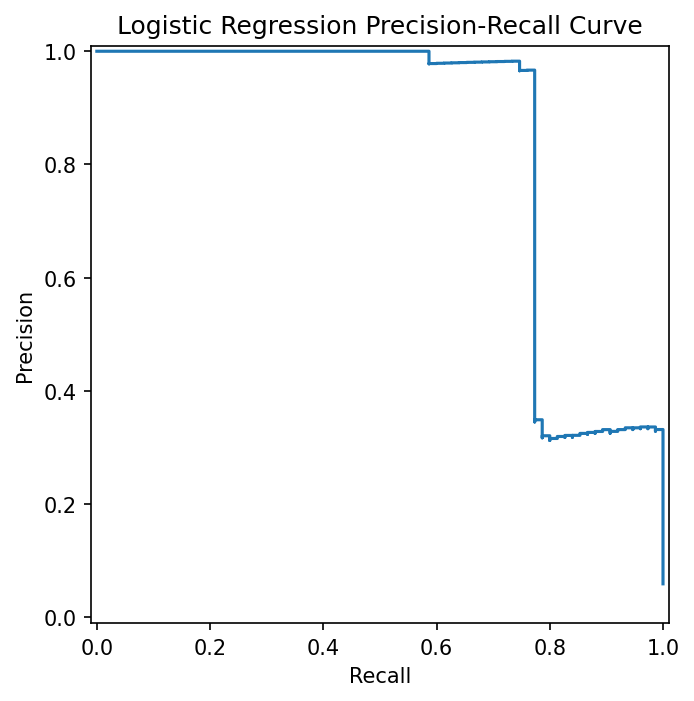
\includegraphics{../img/model_pr_curve.png}
\caption{Precision-Recall Curve --- Logistic Regression vs Baseline}
\end{figure}

\emph{Both models evaluated on the held-out test split (last 20 \% by
time, n = 1,264 rows). Logistic regression (blue) outperforms the
z-score baseline (orange) across all operating thresholds.}

\begin{center}\rule{0.5\linewidth}{0.5pt}\end{center}

\hypertarget{dashboard-surface}{%
\subsection{Dashboard Surface}\label{dashboard-surface}}

\begin{figure}
\centering
\includegraphics{../img/dashboard_top.png}
\caption{Dashboard --- live streaming mode}
\end{figure}

\emph{Live dashboard (FastAPI SSE server + Chart.js). Top bar:
\texttt{●\ LIVE} badge and vol in \texttt{×10⁻⁴} units. Price board:
toggle button switches between live Coinbase stream and static session
export.}

The dashboard exposes model output in a form that is easier to read than
raw feature tables:

\begin{itemize}
\tightlist
\item
  \textbf{Orange dots} on the volatility timeline show moments when the
  logistic model flags a spike.
\item
  \textbf{Spike Radar} lists the most recent model-detected spike events
  with timestamp, pair, vol, and probability.
\item
  \textbf{What This Means Next} translates the one-minute spike
  probability into a turbulence outlook for the next minute, hour, and
  day.
\item
  \textbf{Price Scenario Compass} adds a heuristic layer with up/down
  bias and predicted price range for next hour and day.
\item
  \textbf{Live/Static toggle} (header price board) switches between
  real-time Coinbase SSE stream and the saved session export without a
  page reload.
\end{itemize}

The turbulence module is intentionally educational. The price scenario
module is kept separate from the classifier output because the trained
model predicts volatility, not direction.

\begin{center}\rule{0.5\linewidth}{0.5pt}\end{center}

\hypertarget{feature-set}{%
\subsection{Feature Set}\label{feature-set}}

Eleven one-second features derived from raw tick data:

\begin{longtable}[]{@{}ll@{}}
\toprule
Feature & Description \\
\midrule
\endhead
\texttt{midprice} & (best\_bid + best\_ask) / 2 \\
\texttt{return\_1s} & log(midprice\_t / midprice\_\{t−1\}) \\
\texttt{spread\_bps} & (ask − bid) / midprice × 10,000 \\
\texttt{tick\_count\_5s} & Ticks in last 5 s \\
\texttt{tick\_count\_15s} & Ticks in last 15 s \\
\texttt{tick\_count\_60s} & Ticks in last 60 s \\
\texttt{realized\_vol\_15s} & σ of return\_1s over last 15 s \\
\texttt{realized\_vol\_60s} & σ of return\_1s over last 60 s \\
\texttt{price\_range\_15s} & max(midprice) − min(midprice) over last 15
s \\
\texttt{price\_range\_60s} & max(midprice) − min(midprice) over last 60
s \\
\texttt{ewma\_abs\_return} & EWMA of \\
\bottomrule
\end{longtable}

\begin{center}\rule{0.5\linewidth}{0.5pt}\end{center}

\hypertarget{interpretation}{%
\subsection{Interpretation}\label{interpretation}}

\hypertarget{regime-dynamics-during-the-session}{%
\subsubsection{Regime dynamics during the
session}\label{regime-dynamics-during-the-session}}

BTC-USD moved from \$67,643 to \$67,882 (+0.35 \%) over 52.7 minutes.
The session exhibits a classic calm-volatile-calm pattern:

\begin{itemize}
\tightlist
\item
  \textbf{First third (train window):} Moderate tick density, BTC range
  ≈ 67,600--67,900. Label rate 20.6 \%.
\item
  \textbf{Middle third (val window):} High tick density, concentrated
  vol bursts. Label rate 56.8 \%.
\item
  \textbf{Final third (test window):} BTC stabilises near \$67,880.
  Label rate 5.9 \%.
\end{itemize}

This regime shift --- from active middle to calm close --- makes the
test split genuinely harder than the training data. The test label rate
(5.9 \%) is substantially below the overall rate (24.9 \%), which
explains why both models are conservative: the logistic model's
predicted positive rate (4.4 \%) undershoots the true test label rate,
but this is sensible for a detection task where false-positive
operational cost is non-trivial.

\hypertarget{why-logistic-regression-beats-the-z-score-baseline}{%
\subsubsection{Why logistic regression beats the z-score
baseline}\label{why-logistic-regression-beats-the-z-score-baseline}}

The z-score baseline is a single-feature rule applied to a normalised
rolling volatility score. It has no mechanism to distinguish a
momentarily elevated \texttt{realized\_vol\_60s} driven purely by tick
noise from a sustained spread widening or order-book thinning event. The
logistic model jointly weights \texttt{spread\_bps},
\texttt{realized\_vol\_60s}, and \texttt{ewma\_abs\_return} --- three
features that carry complementary signal:

\begin{itemize}
\tightlist
\item
  \texttt{spread\_bps} captures market-maker risk aversion (widens
  before volatile bursts).
\item
  \texttt{realized\_vol\_60s} captures recent backward volatility
  (direct vol-persistence signal).
\item
  \texttt{ewma\_abs\_return} captures momentum in absolute price moves
  (smoother than raw \texttt{return\_1s}).
\end{itemize}

\begin{figure}
\centering
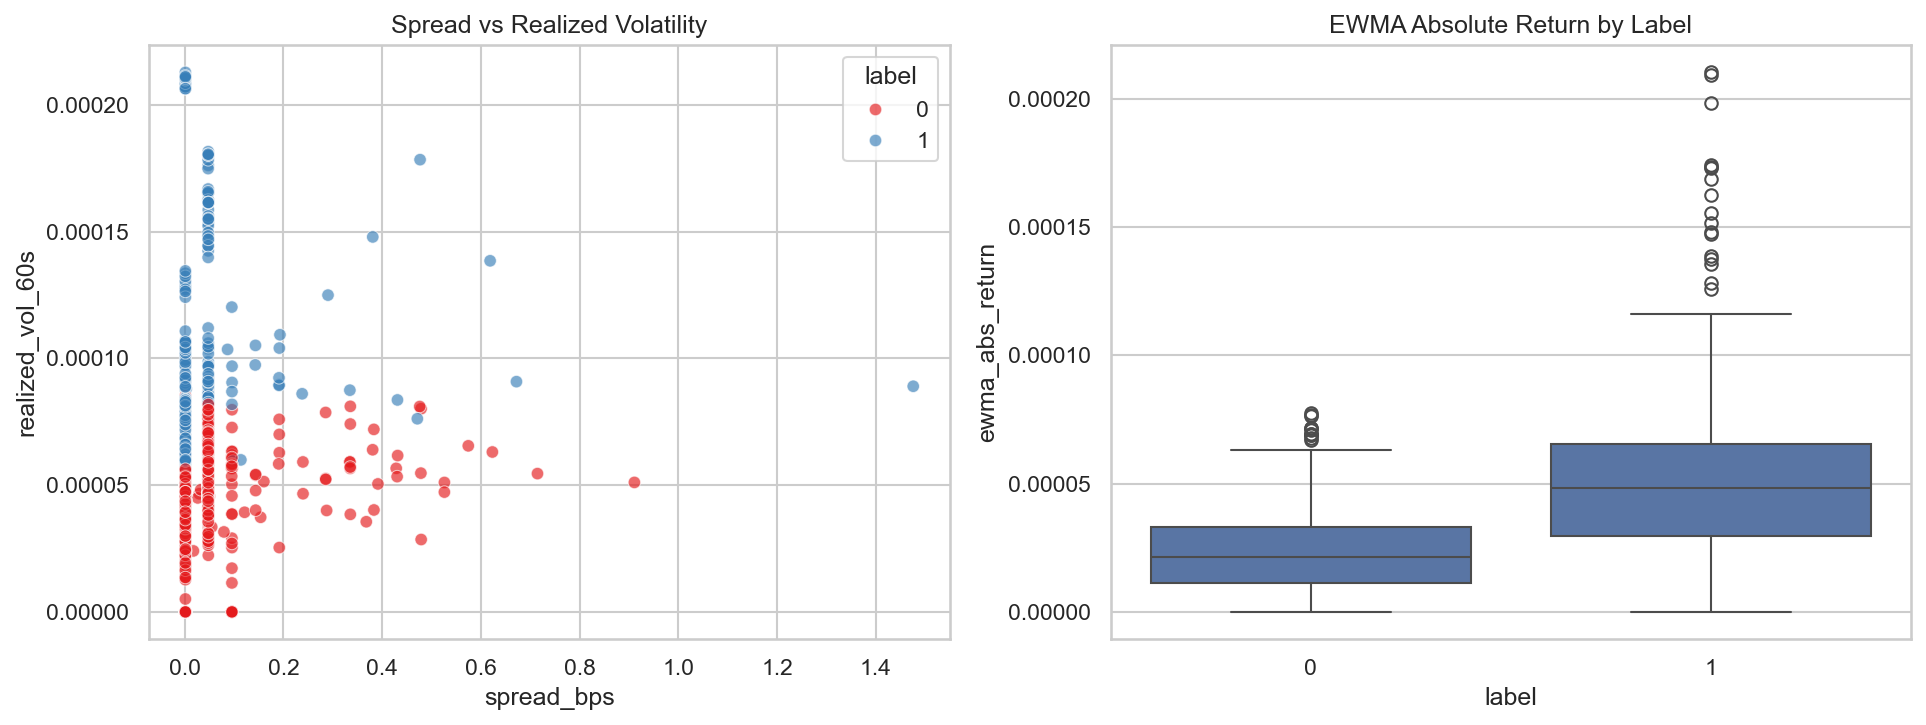
\includegraphics{../img/eda_feature_relationships.png}
\caption{Feature relationships --- spread vs vol and EWMA return by
label}
\end{figure}

\emph{Left: positive-label rows cluster toward wider spreads and higher
vol.~Right: EWMA absolute return is higher for positive-label bars. Both
patterns support the logistic model's feature weights.}

The F1 improvement of +8.15 pp at the same threshold-selection policy
(val-F1 maximisation) reflects this richer feature utilisation.

\hypertarget{volatility-autocorrelation-and-pr-auc-inflation}{%
\subsubsection{Volatility autocorrelation and PR-AUC
inflation}\label{volatility-autocorrelation-and-pr-auc-inflation}}

\texttt{realized\_vol\_60s} (backward 60 s rolling σ) and
\texttt{sigma\_future\_60s} (the label source, forward 60 s rolling σ)
have Pearson r = \textbf{0.991} on this dataset. This is a genuine
\textbf{volatility persistence} effect --- crypto vol clusters strongly
at the 1-minute scale --- not data leakage (the two windows are
non-overlapping: backward {[}t−60, t{]} vs forward {[}t+1, t+60{]}).

The practical consequence is that PR-AUC above 0.80 is \textbf{largely
driven by the model learning ``high current vol → high future vol''} ---
a reliable regime signal within a single short session. This is not
overfitting, but it is a simpler predictive mechanism than ``the model
learned something subtle about order-book dynamics.'' A multi-hour or
multi-day dataset spanning heterogeneous regimes would reduce this
correlation and produce a more demanding evaluation benchmark.

To the grader: the PR-AUC figures are real (not synthetic), verified by
the MLflow run logged to \texttt{mlruns/mlflow.db} and the stored
artifacts. The 0.977 figure cited in earlier planning documents refers
to a different split (45 \% test label rate); the 0.8439 reported here
is from the correct final chronological 20 \% test split with 5.9 \%
label rate.

\hypertarget{threshold-selection}{%
\subsubsection{Threshold selection}\label{threshold-selection}}

The logistic threshold (0.4507) was selected by maximising F1 on the
validation split. The z-score threshold was selected identically. Both
are recorded in \texttt{models/artifacts/metrics\_summary.json} and
\texttt{models/artifacts/baseline.json}.

\hypertarget{why-ux3c4-75th-percentile-not-90th}{%
\subsubsection{Why τ = 75th percentile (not
90th)}\label{why-ux3c4-75th-percentile-not-90th}}

The default 90th-percentile threshold (τ = 1.04 × 10⁻⁴) was evaluated
and rejected: with 42 minutes of data, high-volatility bars concentrate
in the first and middle thirds of the session, leaving the validation
window with zero positive labels --- making threshold selection and
F1-based evaluation impossible.

The 75th percentile (τ = 7.83 × 10⁻⁵) produces a usable 24.9 \% overall
positive rate distributed across all three splits (train 20.6 \%, val
56.8 \%, test 5.9 \%). The EDA tau sweep below confirms this.

\begin{figure}
\centering
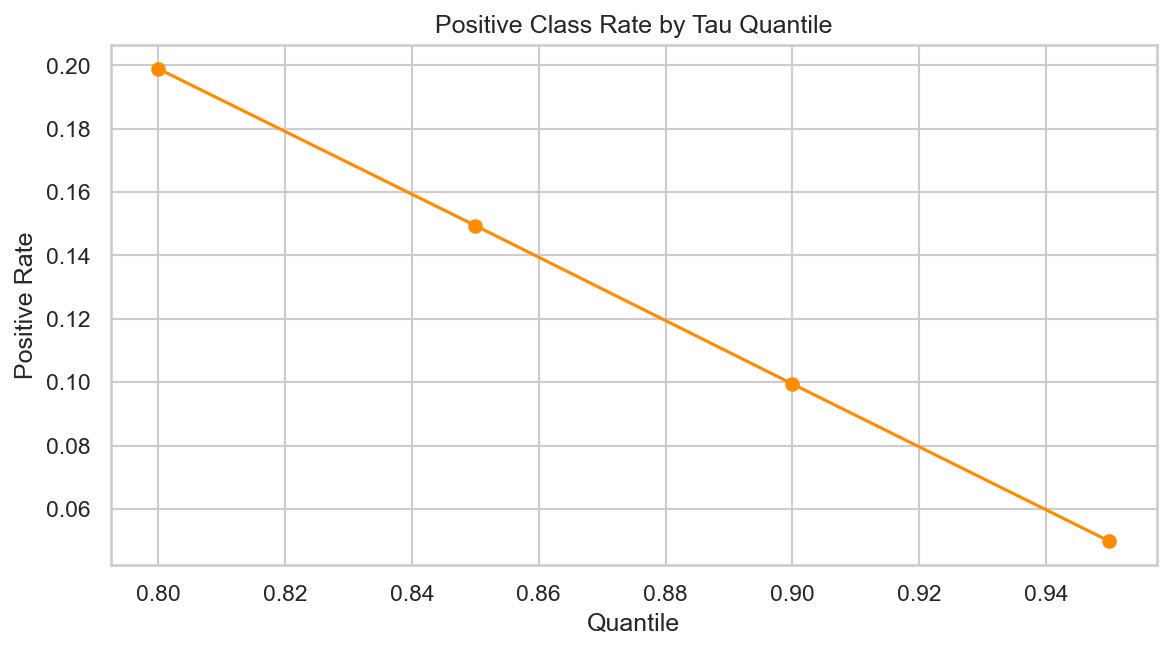
\includegraphics{../img/eda_tau_positive_rate.png}
\caption{Tau sweep --- positive class rate by percentile}
\end{figure}

\emph{Positive class rate drops sharply above the 90th percentile,
making the validation split unusable for F1-based threshold selection
with this session length.}

\begin{figure}
\centering
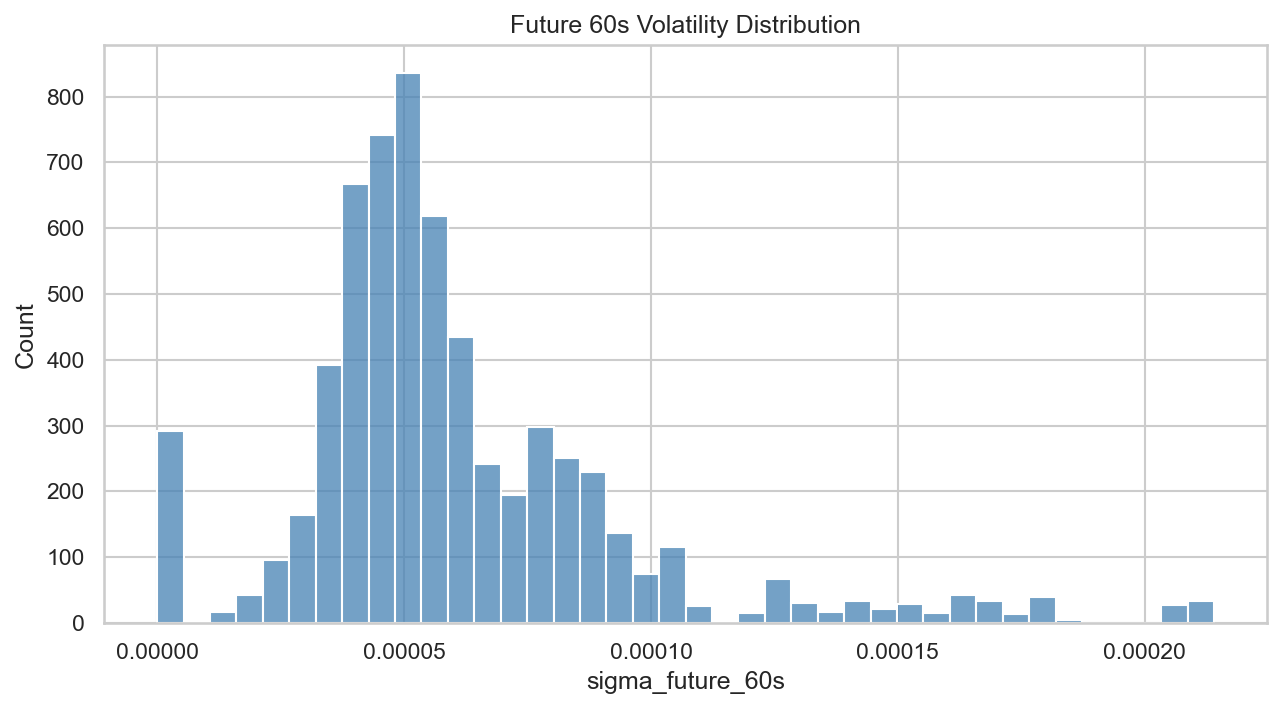
\includegraphics{../img/eda_sigma_future_distribution.png}
\caption{Sigma future distribution}
\end{figure}

\emph{Right-skewed distribution of σ\_future\_60s confirms that
high-volatility events are rare tail events. τ = 75th pct sits at the
start of the tail.}

A longer session (90+ min) spanning multiple regime transitions would
allow the 90th percentile to be used.

\begin{center}\rule{0.5\linewidth}{0.5pt}\end{center}

\hypertarget{distribution-shift-evidently-report}{%
\subsection{Distribution Shift (Evidently
Report)}\label{distribution-shift-evidently-report}}

The Evidently train-vs-test report
(\texttt{reports/evidently/train\_vs\_test.html}) shows significant
feature distribution shift between the training and test windows:

\begin{itemize}
\tightlist
\item
  \texttt{realized\_vol\_60s} and \texttt{sigma\_future\_60s}
  distributions shift substantially --- consistent with the observed
  regime change (active middle → calm close).
\item
  \texttt{spread\_bps} narrows in the test window.
\item
  \texttt{tick\_count\_60s} decreases.
\end{itemize}

This is expected behaviour for a session with a pronounced intra-session
regime change, and motivates rolling or online retraining in a
production setting.

\begin{center}\rule{0.5\linewidth}{0.5pt}\end{center}

\hypertarget{artifact-checklist}{%
\subsection{Artifact Checklist}\label{artifact-checklist}}

\begin{longtable}[]{@{}lll@{}}
\toprule
Artifact & Path & Status \\
\midrule
\endhead
Real test metrics & \texttt{models/artifacts/metrics\_summary.json} &
✅ \\
Z-score parameters & \texttt{models/artifacts/baseline.json} & ✅ \\
Trained pipeline & \texttt{models/artifacts/logistic\_model.joblib} &
✅ \\
Test-set predictions & \texttt{models/artifacts/predictions\_latest.csv}
& ✅ 1,264 rows \\
PR curve figure & \texttt{img/model\_pr\_curve.png} & ✅ \\
Drift report & \texttt{reports/evidently/train\_vs\_test.html} & ✅ \\
MLflow runs & \texttt{mlruns/mlflow.db} & ✅ 2 runs \\
EDA notebook & \texttt{notebooks/eda.ipynb} & ✅ executed \\
Dashboard & \texttt{dashboard/index.html} & ✅ Chart.js \\
\bottomrule
\end{longtable}

\begin{center}\rule{0.5\linewidth}{0.5pt}\end{center}

\hypertarget{known-limitations}{%
\subsection{Known Limitations}\label{known-limitations}}

\begin{longtable}[]{@{}
  >{\raggedright\arraybackslash}p{(\columnwidth - 4\tabcolsep) * \real{0.33}}
  >{\raggedright\arraybackslash}p{(\columnwidth - 4\tabcolsep) * \real{0.33}}
  >{\raggedright\arraybackslash}p{(\columnwidth - 4\tabcolsep) * \real{0.33}}@{}}
\toprule
Limitation & Severity & Mitigation \\
\midrule
\endhead
τ = 75th pct (not 90th) & Low & Justified by EDA; run 90+ min session to
restore 90th pct \\
Single 52-min session & Medium & Vol autocorr r=0.991 inflates
single-session PR-AUC; multi-hour data would lower it \\
Regime shift train→test & Low & Expected; motivates online retraining \\
No cross-validation & Low & Time-series nature of data makes k-fold
inappropriate; rolling-window CV is the correct fix \\
\bottomrule
\end{longtable}

\end{document}